\section{Methodology}
\label{sec:methodology}


\subsection{Data Preprocessing}
In some situations, it becomes difficult to measure the physical properties of a particle such as momentum and energy accurately. In our original dataset, as many as 177000 out of 250000 instances had missing attributes. We considered three approaches to deal with missing values. First, we tried ignoring instances with missing attributes. But this resulted in very few useful instances. Second, we tried to replace the missing values with the mean/median. However, this biases the experiments. Finally, we decided to adopt a method known as multiple imputations~\cite{MultipleImputation} which replaces the missing values with a random number that follows the distribution for that attribute. We use the \texttt{Amelia}~\cite{Amelia} package to perform this task.



\subsection{Feature Engineering and Selection}

\begin{figure*}[t]
\centering
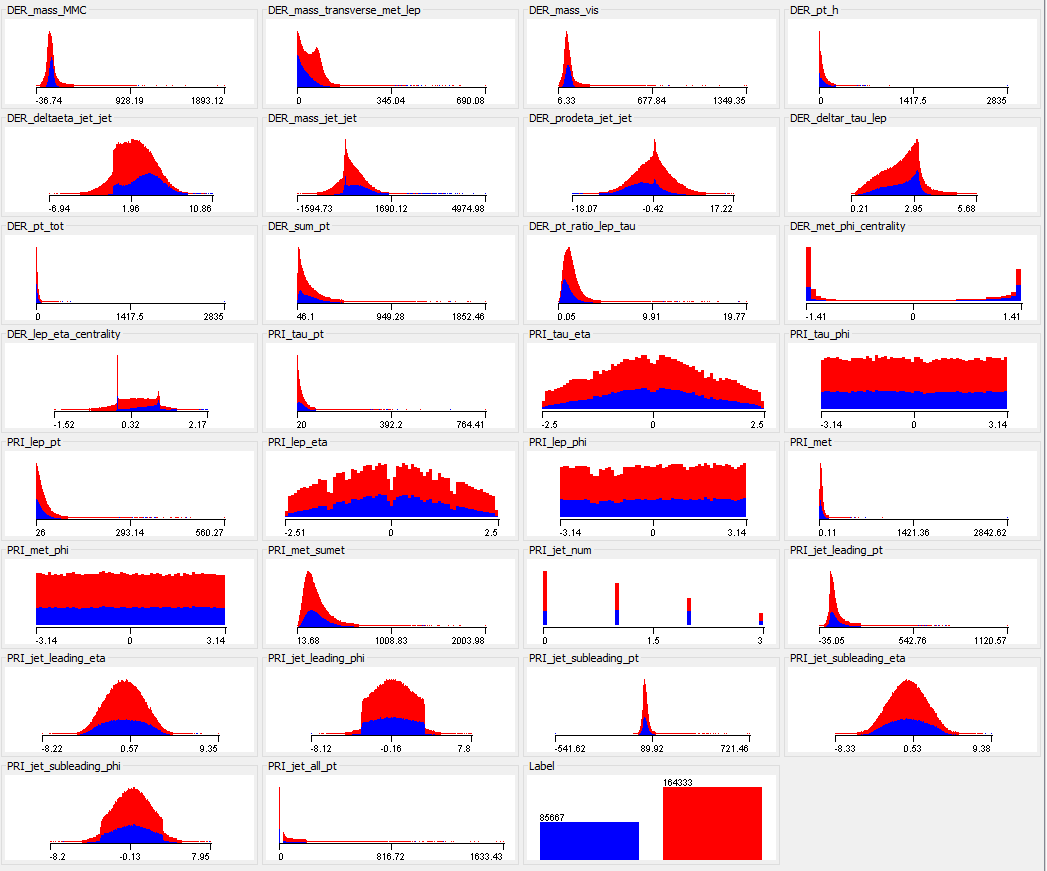
\includegraphics[width=1.8\columnwidth]{Distribution}
\caption{Distribution of different attributes for signal. Blue represents signal and red represents background.}
\label{fig:distribution}
\end{figure*}

The raw dataset includes 17 features. From these 17 basic features, 13 additional features were derived. These 13 derived features describe some property of the particle and requires knowledge of physics. The features are provided by physics. Their description is given in the appendix. From these 30 features, a subset is selected based on the following factors. First, we decide the ability of the feature/attribute to distinguish between signal an background. The distribution of different attributes is shown in Fig.~\ref{fig:distribution} for signal and background separately. Second, we try to avoid using features correlating with each other while building the classifier. Fig.~\ref{fig:correlation-matrix} shows the correlation matrix of the features. The final set of features selected differs for each classifier. The details are given in their respective subsections.

\begin{figure}[h]
\centering
\includegraphics[width=1.0\columnwidth]{corr}
\caption{Correlation matrix. Dark blue indicates features that shows strong positive correlation. Dark red indicates features that show strong negative correlation.}
\label{fig:correlation-matrix}
\end{figure}



\subsection{Data Analytics Techniques}

In this section, we describe the various classification schemes we explored. For each technique, we also describe the parameter settings explored in brief.


\subsubsection{Bayesian Classifiers}

\paragraph{Naive Bayes}

This classifier is based on the Naive Bayes technique developed by John et al.~\cite{NaiveBayes}. In this technique <describe technique here>. <Describe parameter tuning here>.

\subsubsection{Functions-based Classifiers}

\paragraph{Logistic Regression}

This classifier is based on the Ridge estimation technique developed by Cessie et al.~\cite{Logistic Regression}. In this technique <describe technique here>. <Describe parameter tuning here>.

\paragraph{Linear Discriminant Analysis}

\paragraph{Quadratic Discriminant Analysis}



\subsubsection{Tree-based Classifiers}

\paragraph{Simple CART}

This classifier is based on the classification and regression trees (CART) technique developed by Brieman et al.~\cite{CART}. In this technique <describe technique here>. <Describe parameter tuning here>.

\subsubsection{Instance-based Classifiers}

\paragraph{k-Nearest Neighbor}

This classifier is based on the k-nearest neighbor (kNN) technique by aha et al.~\cite{kNN}. In this technique <describe technique here>. <Describe parameter tuning here>.


\subsubsection{Deep Learning}


\subsubsection{Meta Classifiers and Ensemble Methods}

\paragraph{Classification via Clustering and Regression}

We simply cluster the raw dataset and mark certain clusters as signal and others as noise. Prediction based on the distance of the new data point to the centroid of the two cluster groups. 

\paragraph{REP Tree with Bagging}

Bagging technique developed by Brieman involves creating several models using different subsets of the training dataset~\cite{Bagging}. Each model does its own classification and they all vote with equal weight to decide on the class. 


\paragraph{Decision Stump tree with ADA Boosting}

Based on ADA Boosting developed by Freund and Schapire~\cite{ADABoosting}. Used in conjunction with Decision Stump Tree classifier.

\paragraph{Decision Stump tree with Multi-Boosting}

Based on the MultiBoosting technique developed by Webb~\cite{MultiBoosting}.




\paragraph{Rotation Forest}

Rotation Forest is an ensemble method developed by Rodriguez et al.~\cite{RotationForest} where several classifiers are combined to produce a highly accurate classifier. 


